\documentclass[11pt]{report}
\usepackage{amsmath,xcolor}
\usepackage[margin=0.5in]{geometry}
\usepackage{hyperref}
\usepackage{amsmath}
\usepackage{pdfpages}
\usepackage{graphicx}

\begin{document}

\begin{center}
	BIOS 669 Final Project Report \\ Madhuri Raman \\ Due: April 30th, 2024
\end{center}

\section*{Introduction}
	In this project, we will be analyzing data from the 2021/2022 season of the UEFA Champions League which is the biggest professional soccer tournament in Europe. The tournament comprises of the top teams from each regional league in Europe from the previous year, so it represents the highest level of the sport across Europe. The data comes from Kaggle which is linked \href{https://www.kaggle.com/datasets/azminetoushikwasi/ucl-202122-uefa-champions-league?select=distributon.csv}{\textbf{here}}. It contains multiple datasets, each containing important player information, team information, and statistics about a different aspect of the game throughout the tournament. Specifically, the eight datasets are: \textit{Attacking, Defending, Goalkeeping, Goals, Attempts, Disciplinary, Distribution, Key Stats}. \\ \\
	The purpose of this project is to play the role of a data analyst for Real Madrid, who is one of the teams in the Champions League. Although Real Madrid won the Champions League in the 2021/2022 season, our task is to create a report for the players, coaching staff, and scouting team that discusses interesting and notable statistics from the past season of play. We want to see where our club and players stand with respect to the other clubs in terms of both the good and the bad. We may also be interested in which players and clubs are our biggest competition in certain areas of the sport, as well as who should be considered underdogs, dark horses, or maybe even overrated. Although there are a number of interesting questions we could ask about the data, we will focus on three general areas to investigate in this project. These are:
			\begin{itemize}
				\item [1.] Goalkeeper analysis for the scouting team
				\item [2.] Goals and tackle analysis for defenders
				\item [3.] Passing, assists, and shots analysis for attackers
			\end{itemize}
		We go into depth about each of these areas and specify relevant questions of interest in the following sections. Below each question, we provide a table along with a brief answer to the question. Given our audience, we need to keep each answer straightforward and to the point. The players and staff simply look to our analysis as guidance when making their own decisions about the game. \\\\
		We will utilize SAS and several skills learned in BIOS 669 to complete this task, including PROC SQL, PROC REPORT, derived variables, joins, and macros. All code for generating the figures and tables below can be found in the ZIP file containing this report.
\section*{1. Goalkeeper analysis for the scouting team} 

Question of interest for scouting team:
	\begin{itemize}
		\item \textit{Our current goalkeeper (Thibaut Courtois) is out with an ACL injury, and we are in search of a temporary replacement for next year. To do this, we will analyze goalkeepers in the Champions League last year based on the three key metrics present in the goalkeeping data set. In particular, we want to know which goalkeepers had the most saves per match, conceded the least goals, and had the most clean sheets (games where they concede no goals). Ideally, we want to target the best performing goalkeeper in terms of all of these metrics, but the scouting team does prioritize the metrics by the order of them mentioned previously.}
			\begin{center}
				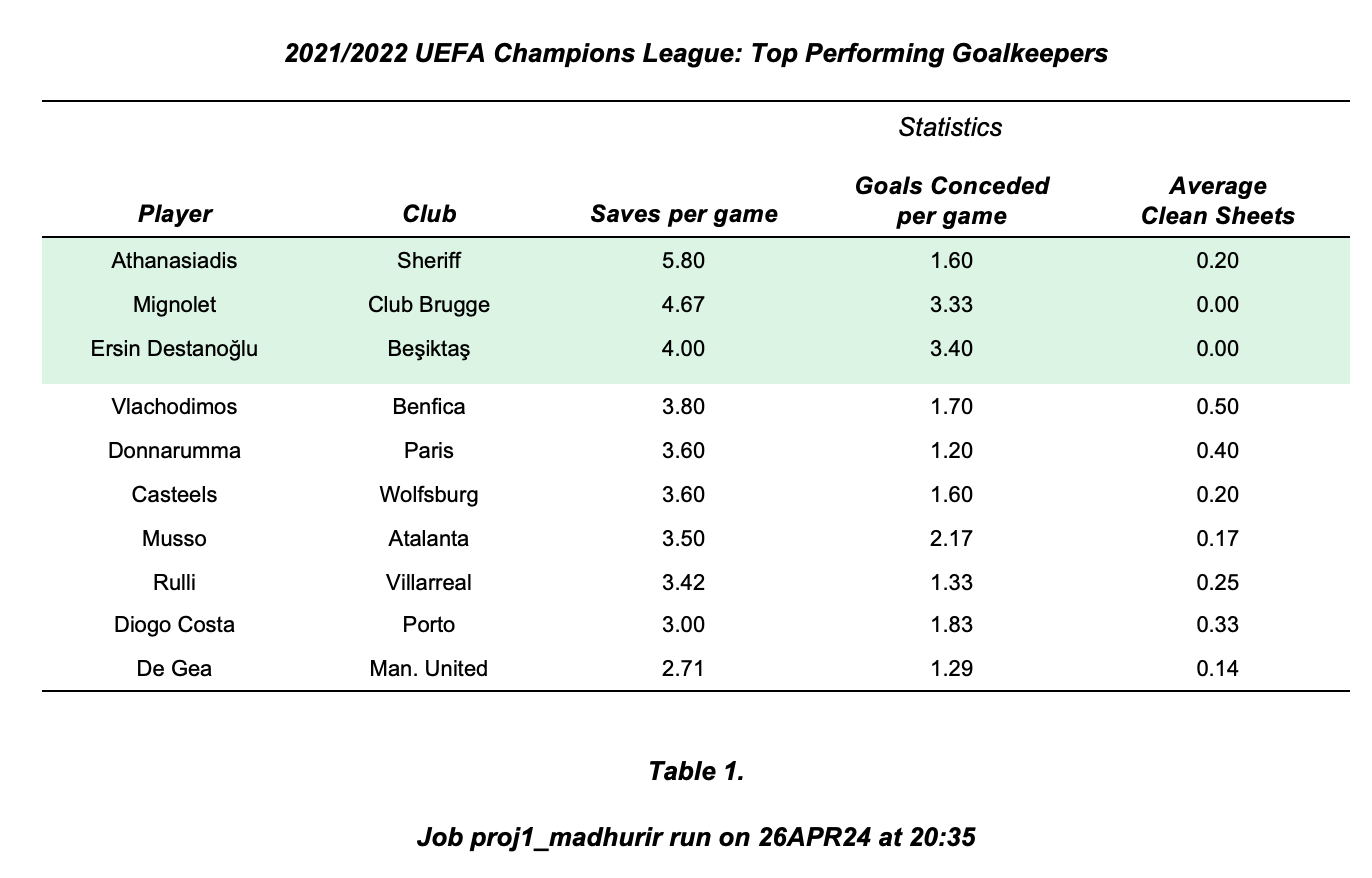
\includegraphics[width=0.9\textwidth]{images_for_report/table1}
			\end{center} 
			
			Based on Table 1, we see that the top three goalkeepers in the Champions League that have played at least five games, based on statistics alone, are Athanasiadis of Club Sheriff, Mignolet of Club Brugge, and Ersin Destanoglu of Besiktas. It is interesting to note that these top three keepers (and most of the keepers in this top ten list) are actually not the most famous or well known, and they don't play for the biggest teams either. This is great news because it means that we can likely buy a good goalkeeper for a fairly cheap price from these clubs. Although these goalkeepers play for not well known clubs, their statistics in the Champions League are evidence that they are capable of performing at the highest level, which is what we need from a replacement for Courtois.  
	\end{itemize}
	
	
	

\section*{2. Goals and tackle analysis for defenders} 
Questions of interest for defenders:
	\begin{itemize}
		\item \textit{What is the most common type and area of goal scored by each team in the tournament? In other words, what kinds of goals should we be wary of?} \\ \\
			In Table 2 below, we see the most common type of goal scored by each team in the Champions League 2021/2022 season, both by types of goals and the areas the goals were scored from. We also see the specific break down of goals per team by type and area. Not surprisingly, most teams' goals were scored from inside the penalty area, which makes sense since it is closer to the goal. Most teams seem to prefer scoring with their right foot, although about 8 teams prefer scoring with their left foot more and two teams, Sheriff and Besiktas, have scored the most by headers. These details are good for the defenders to know when preparing for each opponent next year, since they can try to predict which players and shots are the most dangerous. 
			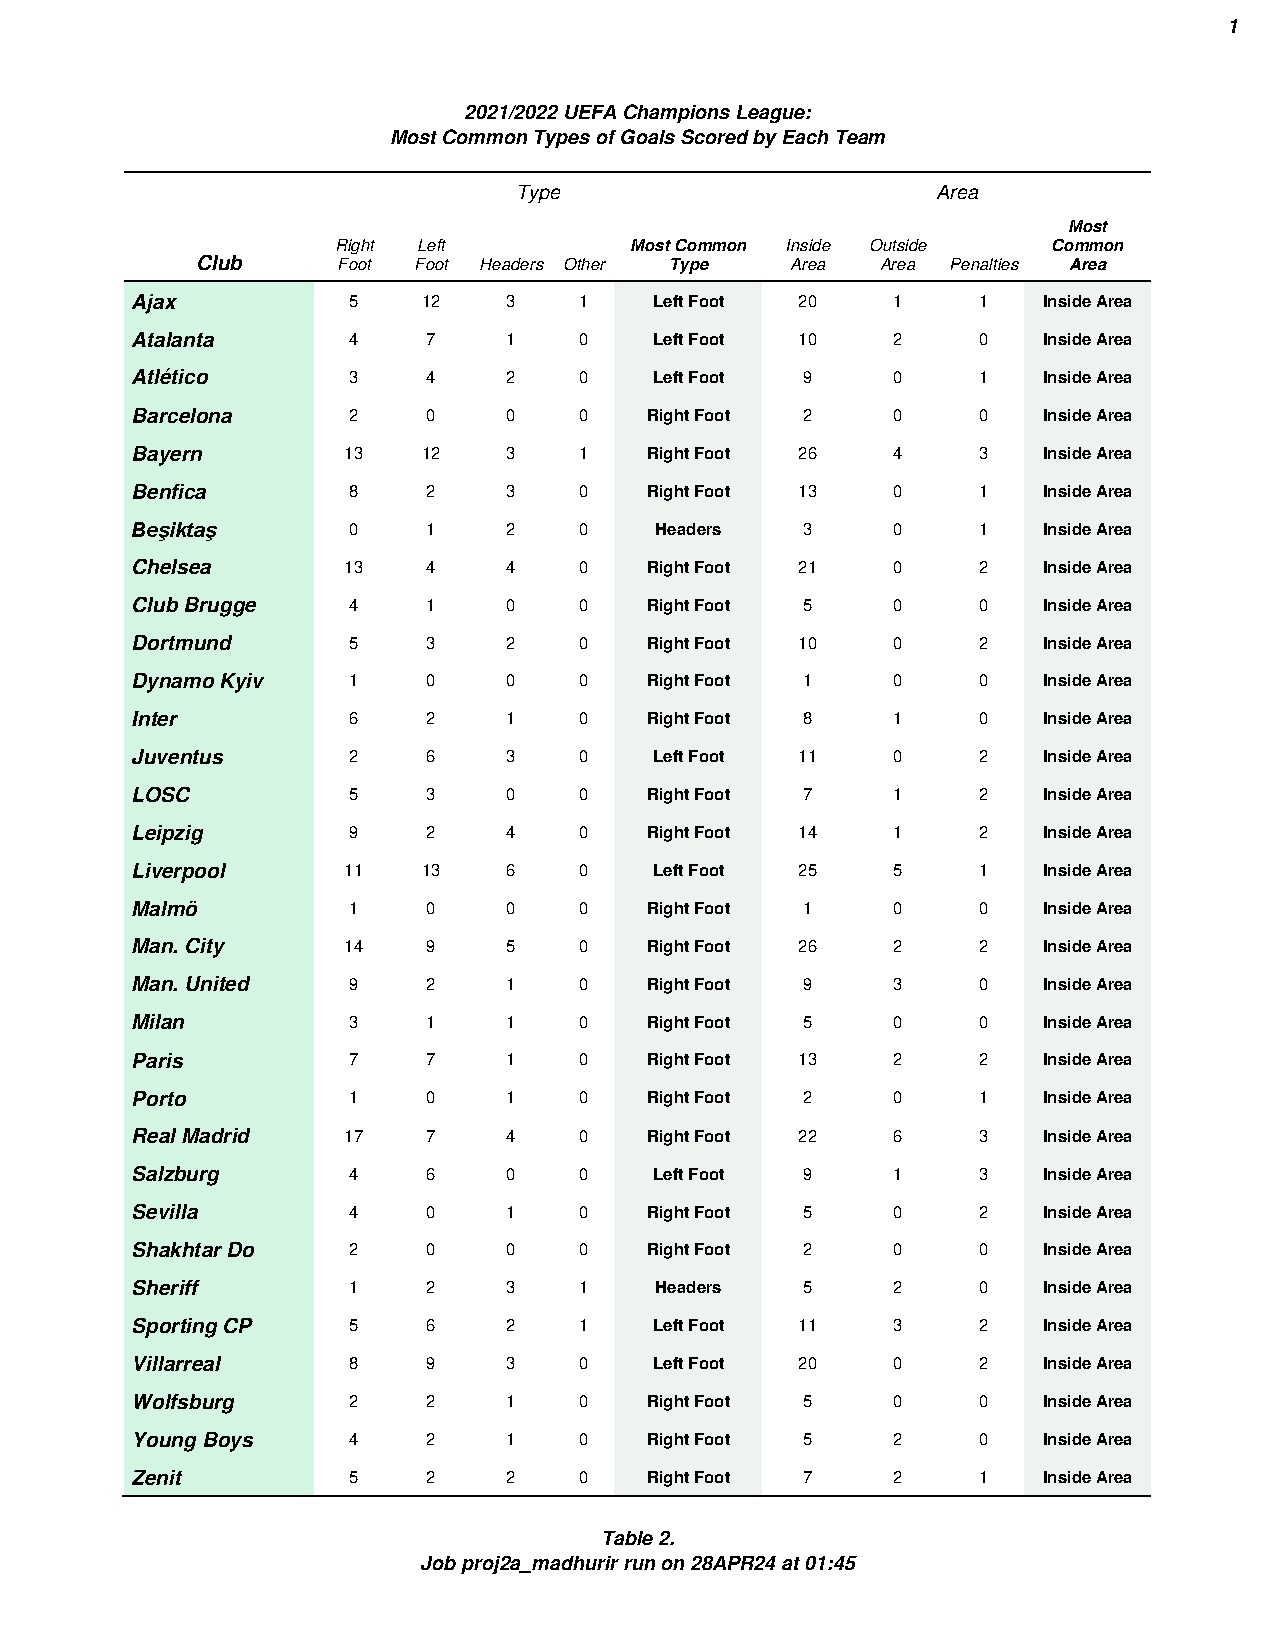
\includepdf{images_for_report/table2.pdf}
			\item \textit{Who is the best at tackling on our team? In other words, who wins the highest percentage of tackles and who wins the most tackles on average per match? What about tackle attempts?}
			\begin{center}
				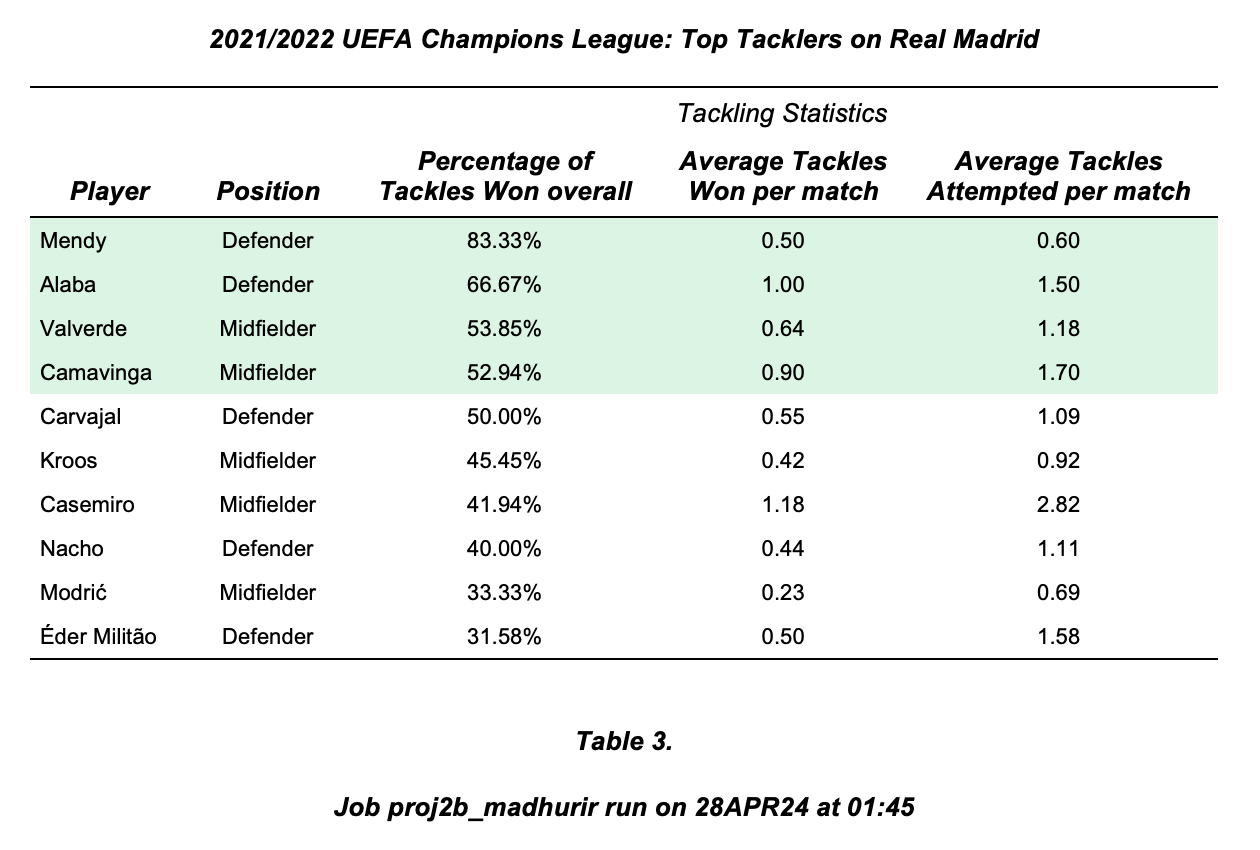
\includegraphics[width=0.9\textwidth]{images_for_report/table3}
			\end{center} 
			We see from Table 3 above an ordered list of the best tacklers on our team (Real Madrid). Specifically, we calculated the percentage of tackles won overall, average tackles won per match, and average tackles attempted per match for each player on the team and ranked the players in order of percentage of tackles won overall. We highlight in green the players with over 50\% of tackles won overall. Based on this, Ferland Mendy is the best tackler on the team in this Champions League season. It is also great to see that even though this was Eduardo Camavinga's first season on Real Madrid at 19 years old, and even though he is a midfielder, he was a great tackler in this tournament. This is probably why he has recently been playing in defensive positions with David Alaba out with an ACL injury as well He is a very promising and flexible young player! On the other hand, Eder Militao and Nacho are two defenders with a bit worse tackle winrates, so perhaps this is an area that they can focus on improving.
	\end{itemize}

\section*{3. Passing, assists, and shots analysis for attackers}
Questions of interest for attackers (midfielders and forwards):
	\begin{itemize}
		\item \textit{Who, on our team, has the best ratio of shots on target to shots off target? In other words, who is more likely to shoot on target when they take a shot?}
			\begin{center}
				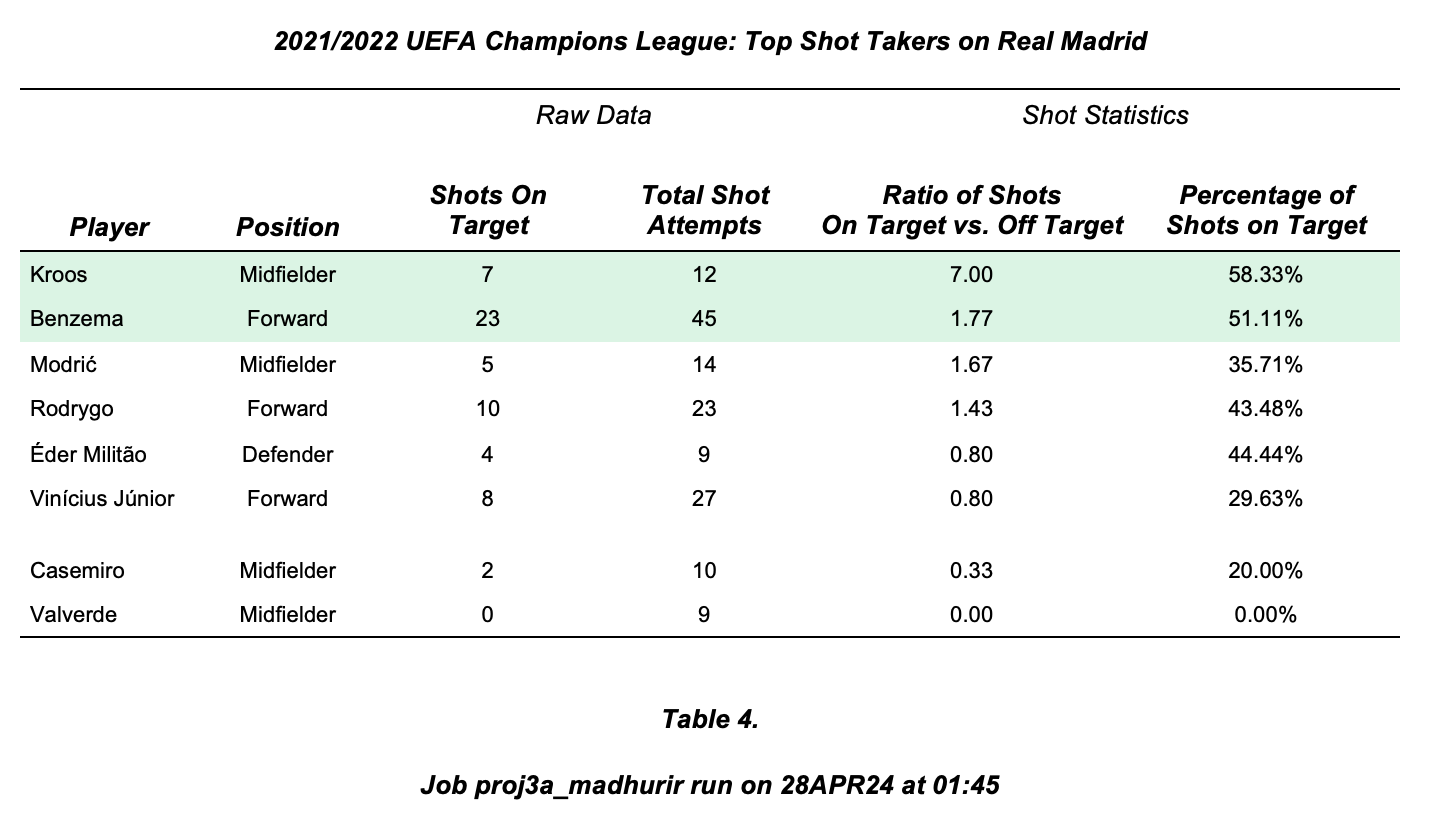
\includegraphics[width=0.9\textwidth]{images_for_report/table4}
			\end{center} 
			Table 4 shows the top shot takers for Real Madrid and highlights the two players with over 50\% of shots on target on average. Karim Benzema is one of the best players in the world and won the Ballon d'or (best player in the world of the year) right after this Champions League season, so the quality of his shots is not surprising at all. Toni Kroos is a highly experienced and talented midfielder, so we are also not surprised to see him top the list with seven shots on target to every one shot off target in the Champions League. Based on these statistics, we see that Vini Jr. and Valverde enjoy taking a of shots but most are not on target, so this can definitely be an area of improvement for them.
		\item \textit{Who had the most assists per game and most passes completed per game in the league overall? What about from our team? And are these lists the same? In other words, are players who assist the most goals also the best passers in general during a game? This will help inform our game strategy.} \\ \\
			Finally, we examine Table 5 below which contains a list of the top 30 best passers in this Champions League season along with their respective number of assists, for all players with at least five matches played. This list is sorted by overall pass accuracy (total passes completed / total passes attempted) followed by average number of passes completed per game. Pass accuracy is an indicator of the quality of their passes, and average passes completed per game is an indicator of the actual number of good passes they make (quantity). \\\\
			Before this analysis, we hypothesized that the best passers may also be more likely to assist goals, due to both the quantity and quality of their passes. However, we clearly see from this table that the players with highest pass accuracy (highlighted in grey) all have only one assist in this Champions League season. They have both quantity and quality of passes but very low assist numbers. When we think about this some more, it actually makes sense. During a soccer game, defenders often try to slow down the game and "regroup" by keeping the ball in their half of the field and passing slowly between each other and their goalkeeper, before making an attacking play. They are rarely ever contested by opposing players when doing this, which explains why their pass accuracy is so high. Additionally, it is rare for defenders to assist goals by nature of their role and position on the field, which explains the low number of assists. We also see our players bolded in this list. Ferland Mendy, who was our top tackler, is fairly high on this list (top 10) based on pass accuracy and has two assists. Luka Modric is also on this list with high pass accuracy and four assists as well. This is not surprising at all because like Toni Kroos, Modric is a very experienced player often nicknamed "the magician", so his passes as a midfielder are more likely to be contested by opposing defenders but are still very high quality!
			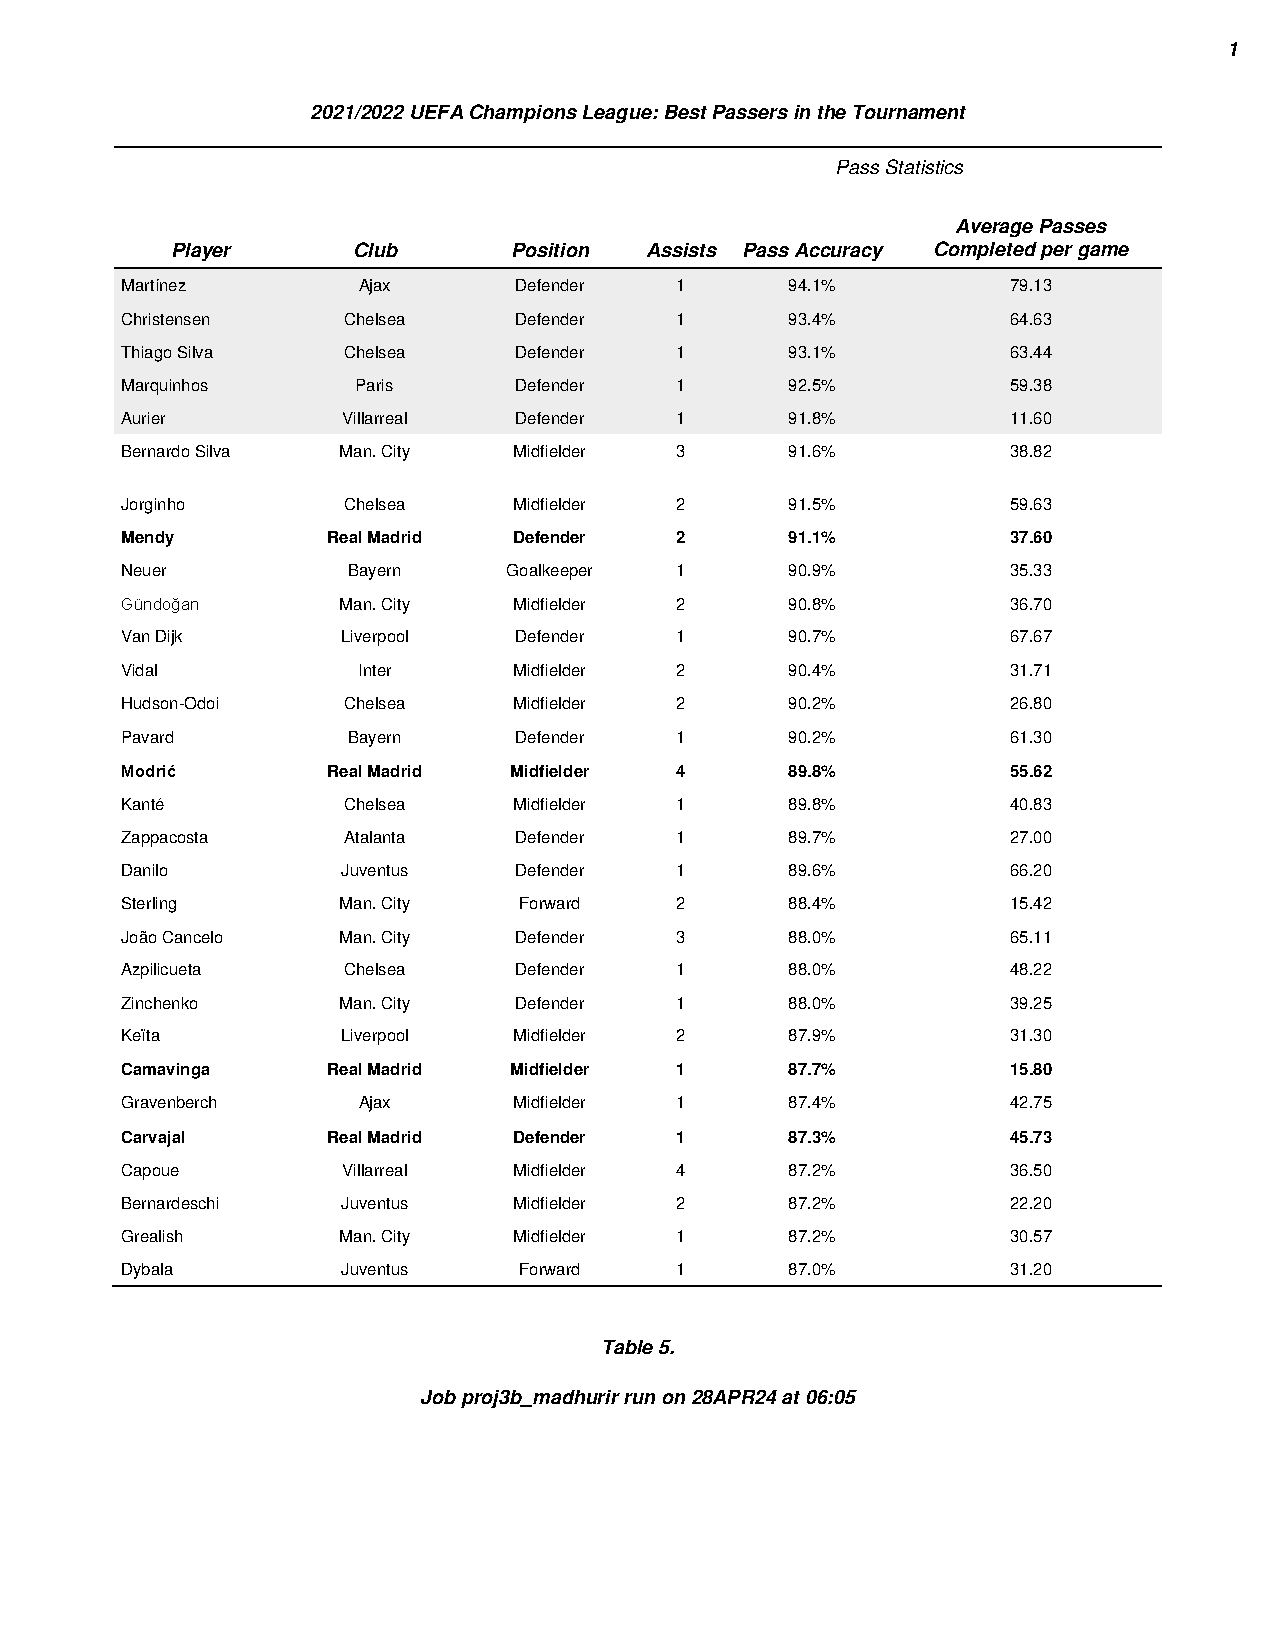
\includepdf{images_for_report/table5.pdf}
	\end{itemize}

\section*{Conclusion}
In this project, we conducted data analysis of UEFA Champions League data from the 2021/2022 season as an analyst for the club Real Madrid. We utilized tools in SAS that we learned from BIOS 669, including PROC SQL, PROC REPORT, joins, derived variables, etc. We created several reports to address questions of interest from a variety of people on the team. Specifically, our analysis benefitted/was for the scouting team, the defenders, and the attackers on the team. We hope that the key takeaways we summarized for each question and table will be useful for the team's improvement and decision-making for next season. 

\end{document}